\documentclass[11pt,a4paper]{article}
\usepackage[left=24mm,right=24mm,top=20mm,bottom=20mm,headheight=14pt]{geometry}
\usepackage[T1]{fontenc}
\usepackage{lmodern}
\usepackage{microtype}
\usepackage{amsmath,amssymb,amsthm}
\usepackage{graphicx}
\graphicspath{{figures/}}
\usepackage{booktabs}
\usepackage{fancyhdr}
\usepackage{xcolor}
\usepackage{tikz}
\usetikzlibrary{arrows.meta}
\usepackage[colorlinks=true,linkcolor=blue!50!black,citecolor=blue!50!black,urlcolor=blue!50!black]{hyperref}
\usepackage{caption}
\captionsetup{font=small,labelfont=bf}
\setlength{\parindent}{1.5em}
\setlength{\parskip}{0pt}
\setlength{\textfloatsep}{12pt plus 2pt minus 2pt}
\setlength{\intextsep}{12pt plus 2pt minus 2pt}
\pagestyle{fancy}
\fancyhf{}
\fancyhead[L]{\small Hawking--Bondi thermal feedback}
\fancyhead[R]{\small E. Anaraly uulu}
\fancyfoot[C]{\thepage}
\renewcommand{\headrulewidth}{0.3pt}
\newtheorem{proposition}{Proposition}
\newcommand{\Pbb}{P_{\mathrm{bb}}}
\newcommand{\Mc}{M_{c0}}
\newcommand{\tstar}{t_*}
\newcommand{\Cenv}{C_{\mathrm{env}}}

\begin{document}
\begin{center}
{\LARGE\bfseries Thermal Feedback in a Microscopic\\[2pt] Black Hole Reactor\par}
\vspace{5pt}
{\large Stability of a coupled Hawking--Bondi model\par}
\vspace{13pt}
{\normalsize Emir Anaraly uulu\par}
Independent Researcher, Bishkek, Kyrgyz Republic\\
\href{mailto:anarem1004@gmail.com}{\texttt{anarem1004@gmail.com}}\\[7pt]
Original manuscript: 30 September 2026 \quad\textbar\quad Revised: 22 October 2026
\end{center}
\vspace{4pt}

\begin{abstract}
In a fixed medium, the balance between idealized Bondi accretion and blackbody Hawking evaporation of a microscopic black hole is unstable. We ask whether heating of the medium by the hole's own radiation can stabilize it. The black-hole mass is coupled to an effective temperature of the surrounding gas: the ideal-gas sound speed makes the Bondi coefficient scale as $T^{-3/2}$, while deposited Hawking power and linear cooling set the temperature. The resulting two-variable system has exactly one positive equilibrium, hotter and more massive than the fixed-medium balance. Its Jacobian determinant is negative for every positive heating and cooling strength, so the equilibrium is a saddle. The same holds for any one-zone model in which heating decreases with mass, accretion decreases with temperature and cooling increases with temperature. Thermal coupling raises the growth rate of perturbations relative to a frozen temperature at the same equilibrium, although the shifted equilibrium departs more slowly than the fixed-medium one. Order-of-magnitude estimates for two hydrogen plasmas show that neither meets the conditions under which a one-zone thermal reservoir would describe the flow at the balance mass.
\end{abstract}

\section{Introduction}
In a previous paper~\cite{paperI} we balanced idealized Bondi accretion against a blackbody approximation to Hawking evaporation,
\begin{equation}
 \dot M = AM^2-\frac{B}{M^2},\qquad A,B>0,
 \label{eq:paperI}
\end{equation}
and showed that its only positive balance, $\Mc=(B/A)^{1/4}$, is unstable: the right-hand side increases with mass, so a perturbation of either sign grows. In dimensionless form every case reduces to $dx/ds=x^2-x^{-2}$, whose fixed point $x=1$ has growth rate~4.

That analysis held the density and sound speed of the medium fixed. This is a strong restriction, because the hole is itself a powerful heat source: at the reference balance mass of Ref.~\cite{paperI}, its blackbody luminosity is $3.6\times10^{11}$~W. Heating raises the sound speed, and the Bondi rate falls as its inverse cube. The question of the present paper is therefore:
\begin{quote}
\itshape Can heating of the accreting medium by Hawking radiation turn the repelling balance into an attracting one?
\end{quote}

Recent time-dependent calculations of primordial black holes accreting inside stars show that the thermodynamics of the inflowing gas can change the classical adiabatic Bondi rate substantially~\cite{cantiello}. Their luminosity comes from the accreting gas rather than from Hawking emission, so we take from them only the modeling principle: the thermal state of the medium should be allowed to evolve and feed back on accretion.

We add the smallest ingredient that makes this question testable: one effective temperature $T(t)$ of the medium, evolving together with $M(t)$ at fixed density. Section~\ref{sec:model} sets up the model and Sec.~\ref{sec:equilibrium} locates its equilibrium. Section~\ref{sec:stability} proves that the equilibrium is a saddle for all positive parameters, compares three growth rates that are easily confused, and extends the result to a class of monotone heating and cooling laws. Section~\ref{sec:numerics} checks these statements numerically, and Sec.~\ref{sec:physical} estimates whether any simple plasma could support the one-zone description.

Throughout, the black hole is uncharged and nonrotating, the emission follows the photon-blackbody baseline of Ref.~\cite{paperI}, and ``stability'' refers to the equilibrium of the stated differential equations. The word ``reactor'' names the motivating question of this series; confinement, energy collection and engineering feasibility are outside its scope.

\section{Model}\label{sec:model}
\subsection{Accretion and evaporation}
For a Schwarzschild black hole the Hawking temperature scales as $T_H\propto M^{-1}$~\cite{hawking}. Treating the horizon as a photon blackbody gives
\begin{equation*}
 \Pbb=\frac{K}{M^2},\qquad K=\frac{\hbar c^6}{15360\pi G^2},\qquad
 \dot M_{\rm evap}=-\frac{B}{M^2},\qquad B=\frac{K}{c^2}.
\end{equation*}
This is a simplified baseline: greybody factors and the additional particle species available at high temperature change the emission rate~\cite{page,macgibbon}.

Steady spherical Bondi accretion of a gas at rest far from the hole gives~\cite{bondi}
\begin{equation*}
 \dot M_{\rm acc}=A\,M^2,\qquad A=\frac{4\pi\lambda\rho_\infty G^2}{c_s^3}.
\end{equation*}
For an ideal gas with fixed composition and adiabatic index, $c_s^2=\gamma k_BT/(\mu m_p)$. At fixed density $\rho_\infty$ and accretion parameter $\lambda$, the coefficient therefore depends on temperature as
\begin{equation}
 A(T)=A_0\left(\frac{T}{T_0}\right)^{-3/2}.
 \label{eq:AT}
\end{equation}

The temperature $T$ must describe the gas that sets the Bondi boundary condition, at radii of order the Bondi radius and beyond. Heating only a thin layer near the horizon would not change that boundary condition. We therefore assume a well-mixed reservoir in which deposited radiation reaches the gas that controls accretion. This is a closure assumption; Sec.~\ref{sec:physical} examines when it could hold.

The water-like reference medium of Ref.~\cite{paperI} is not an ideal gas and does not define a consistent $T_0$. We use its balance mass and time unit only as scales and calibrate no thermal parameter to water.

\subsection{Heating and cooling}
Let a fraction $\epsilon$ of the blackbody luminosity be deposited in a reservoir of constant heat capacity $\Cenv$, and let a linear cooling law return the reservoir to $T_0$ on a timescale $\tau_c$. The model is
\begin{equation}
 \dot M=A_0\left(\frac{T}{T_0}\right)^{-3/2}M^2-\frac{B}{M^2},\qquad
 \Cenv\dot T=\frac{\epsilon K}{M^2}-\frac{\Cenv}{\tau_c}(T-T_0),
 \label{eq:dimensional}
\end{equation}
with all constants positive, $0<\epsilon\le1$ and $M,T>0$. The parameters $\epsilon$, $\Cenv$ and $\tau_c$ are not derived from the emission spectrum, opacity or geometry. The reservoir has no spatial structure and does not track the energy carried by gas flowing in and out.

\subsection{The feedback loop}
Equation~\eqref{eq:dimensional} contains a single closed loop (Fig.~\ref{fig:loop}). A decrease of $M$ raises $\Pbb$; the deposited power heats the reservoir; the higher sound speed lowers $A(T)$; and the weaker accretion lets evaporation remove mass faster. The loop therefore reinforces the initial perturbation. A complete description would also include the response of the density and a transport delay between the deposition region and the Bondi radius. Neither is modeled here: holding $\rho_\infty$ fixed isolates the sound-speed channel.

\begin{figure}[tbp]
\centering
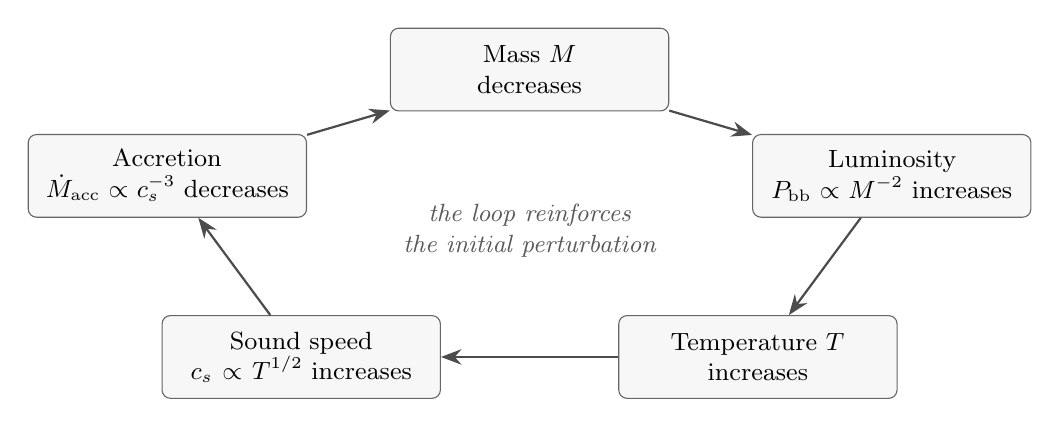
\begin{tikzpicture}[
  box/.style={draw=black!60, rounded corners=3pt, fill=black!3, align=center,
              text width=3.3cm, minimum height=1.05cm, font=\small},
  arr/.style={-{Stealth[length=2.6mm]}, thick, black!70}]
 \node[box] (m) at (0,1.9)     {Mass $M$\\decreases};
 \node[box] (p) at (4.6,0.55)  {Luminosity\\$\Pbb\propto M^{-2}$ increases};
 \node[box] (t) at (2.9,-1.75) {Temperature $T$\\increases};
 \node[box] (c) at (-2.9,-1.75){Sound speed\\$c_s\propto T^{1/2}$ increases};
 \node[box] (a) at (-4.6,0.55) {Accretion\\$\dot M_{\rm acc}\propto c_s^{-3}$ decreases};
 \draw[arr] (m) -- (p);
 \draw[arr] (p) -- (t);
 \draw[arr] (t) -- (c);
 \draw[arr] (c) -- (a);
 \draw[arr] (a) -- (m);
 \node[font=\small\itshape, text=black!65, align=center] at (0,-0.15) {the loop reinforces\\the initial perturbation};
\end{tikzpicture}
\caption{\textbf{The thermal feedback loop for a downward mass perturbation.} Every link follows from Eq.~\eqref{eq:dimensional}. An upward perturbation runs the same loop with every change reversed and favors further growth.}
\label{fig:loop}
\end{figure}

\subsection{Dimensionless form}
Let $\Mc=(B/A_0)^{1/4}$ be the fixed-medium balance mass at $T=T_0$ and $\tstar=(A_0\Mc)^{-1}$ its time unit. With $x=M/\Mc$, $\theta=T/T_0$ and $s=t/\tstar$, Eq.~\eqref{eq:dimensional} becomes
\begin{equation}
 \frac{dx}{ds}=F(x,\theta)=\theta^{-3/2}x^2-x^{-2},\qquad
 \frac{d\theta}{ds}=G(x,\theta)=\eta x^{-2}-\zeta(\theta-1),
 \label{eq:system}
\end{equation}
where
\begin{equation}
 \eta=\frac{\tstar\epsilon K}{\Cenv T_0\Mc^2},\qquad
 \zeta=\frac{\tstar}{\tau_c},\qquad
 \chi=\frac{\eta}{\zeta}=\frac{\epsilon\Pbb(\Mc)\,\tau_c}{\Cenv T_0}.
 \label{eq:params}
\end{equation}
The feedback strength $\chi$ compares the energy deposited during one cooling time with the thermal energy scale $\Cenv T_0$ of the reservoir. The cooling rate $\zeta$ compares the cooling time with the mass time unit of the fixed-medium model. The two can be varied independently; changing $\tau_c$ alone changes both.

\section{The shifted equilibrium}\label{sec:equilibrium}
The nullclines of Eq.~\eqref{eq:system} are
\begin{equation*}
 F=0:\ x=\theta^{3/8},\qquad G=0:\ \theta=1+\chi x^{-2}.
\end{equation*}
The first rises with temperature and the second falls with mass, so they intersect once. The intersection $(x_*,\theta_*)$ satisfies
\begin{equation}
 x_*=\theta_*^{3/8},\qquad \theta_*-1=\chi\,\theta_*^{-3/4}.
 \label{eq:equilibrium}
\end{equation}
The function $h(\theta)=\theta-1-\chi\theta^{-3/4}$ is negative at $\theta=1$, grows without bound, and has $h'(\theta)=1+\tfrac34\chi\theta^{-7/4}>0$. Hence for every $\chi>0$ there is exactly one positive equilibrium, with $\theta_*>1$ and $x_*>1$. Its position depends on $\chi$ alone. In the two limits,
\begin{equation*}
 \chi\ll1:\ \theta_*=1+\chi+O(\chi^2),\quad x_*=1+\tfrac38\chi+O(\chi^2);\qquad
 \chi\gg1:\ \theta_*\sim\chi^{4/7},\quad x_*\sim\chi^{3/14}.
\end{equation*}
Heating therefore moves the balance to a hotter medium and a larger mass (Fig.~\ref{fig:equilibrium}a). Whether trajectories return to the shifted balance is a separate question, answered next.

\begin{figure}[tbp]
 \centering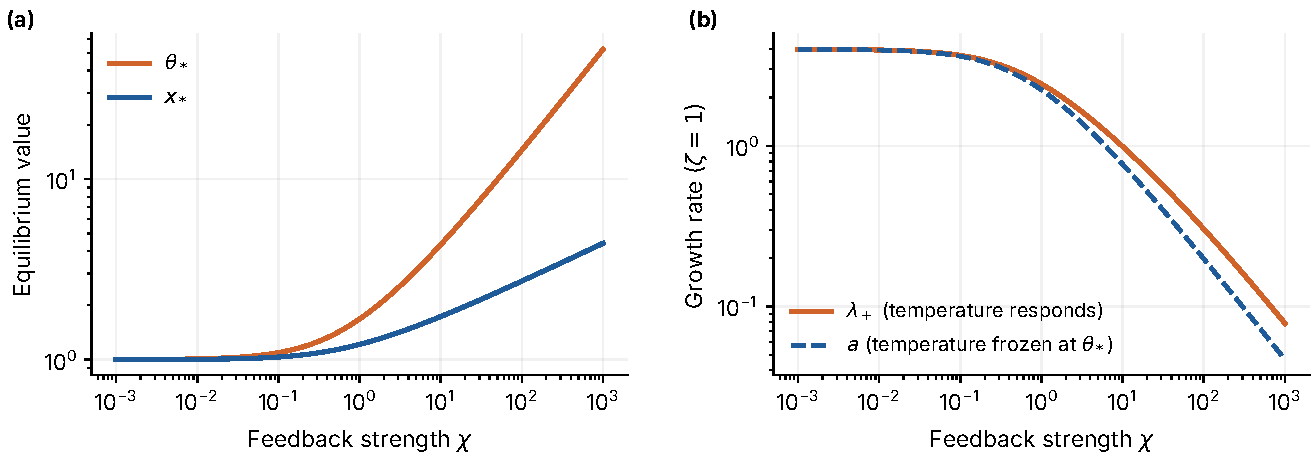
\includegraphics[width=\linewidth]{equilibrium.pdf}
 \caption{\textbf{Heating shifts the balance without making it attracting.} (a) Equilibrium temperature and mass from Eq.~\eqref{eq:equilibrium}. (b) For $\zeta=1$, the unstable eigenvalue $\lambda_+$ of the coupled system and the growth rate $a=4x_*^{-3}$ obtained when the temperature is frozen at $\theta_*$. Both rates fall as the equilibrium moves to larger mass, but $\lambda_+>a$ throughout.}
 \label{fig:equilibrium}
\end{figure}

\section{Linear stability}\label{sec:stability}
\subsection{A saddle for every positive coupling}
The partial derivatives of Eq.~\eqref{eq:system} are
\begin{equation*}
 F_x=2\theta^{-3/2}x+2x^{-3},\quad
 F_\theta=-\tfrac32\theta^{-5/2}x^2,\quad
 G_x=-2\eta x^{-3},\quad
 G_\theta=-\zeta.
\end{equation*}
At the equilibrium $\theta_*^{-3/2}=x_*^{-4}$, so the Jacobian is
\begin{equation*}
 J_*=\begin{pmatrix} a & b\\ c & -\zeta\end{pmatrix},\qquad
 a=4x_*^{-3}>0,\quad
 b=-\tfrac32\theta_*^{-5/2}x_*^2<0,\quad
 c=-2\eta x_*^{-3}<0,
\end{equation*}
with determinant
\begin{equation}
 \det J_*=-4\zeta x_*^{-3}-3\eta\,\theta_*^{-5/2}x_*^{-1}<0.
 \label{eq:det}
\end{equation}
A real $2\times2$ matrix with negative determinant has two real eigenvalues of opposite sign. The equilibrium is therefore a saddle for every $\eta,\zeta>0$. A stable node, a stable focus and a Hopf bifurcation are all excluded, because each requires $\det J_*>0$.

\subsection{Three growth rates}
Three rates are easily confused when judging the effect of heating. The first is $a$, the growth rate of a mass perturbation at the new equilibrium when the temperature is frozen at $\theta_*$. The second is the unstable eigenvalue of the coupled system,
\begin{equation}
 \lambda_\pm=\frac{a-\zeta\pm\sqrt{(a+\zeta)^2+4bc}}{2},\qquad
 \lambda_+>a>0,\qquad \lambda_-<-\zeta,
 \label{eq:eigenvalues}
\end{equation}
where the inequalities follow from $bc>0$. The third is the rate 4 of the fixed-medium balance. For $\chi=\zeta=1$ these are $a=2.234$, $\lambda_+=2.431$ and 4. Letting the temperature respond raises the growth rate at a given equilibrium from $a$ to $\lambda_+$: the coupling itself is destabilizing. The shift of the equilibrium to larger mass lowers all rates, which is why $\lambda_+$ is smaller than 4. A smaller $\lambda_+$ therefore reflects the shifted equilibrium, not a stabilizing effect of the feedback.

The unstable eigenvector has slope $(\lambda_+-a)/b<0$ in the $(x,\theta)$ plane and the stable one has slope $(\lambda_--a)/b>0$. Only initial conditions on the one-dimensional stable manifold approach the equilibrium; a generic perturbation has an unstable component. A loss of mass at the equilibrium temperature, for example, raises the heating term and lowers the accretion coefficient, both of which accelerate further loss.

\subsection{Limiting cases}
For fixed $\zeta$ and $\chi\gg1$, Eq.~\eqref{eq:eigenvalues} gives $\lambda_+\sim7\chi^{-9/14}$ (Appendix~\ref{app:scaling}). The growth rate becomes small but stays positive for every finite $\chi$. At fixed $\chi$, changing $\zeta$ also changes $\eta=\chi\zeta$; the slow- and fast-cooling limits are
\begin{equation*}
 \lim_{\zeta\to0^+}\lambda_+=a,\qquad
 \lim_{\zeta\to\infty}\lambda_+=a+3\chi\,\theta_*^{-5/2}x_*^{-1}>a.
\end{equation*}
In the first limit the temperature cannot respond during a mass e-folding; in the second it follows the mass adiabatically along $G=0$. Neither limit reverses the instability.

\subsection{A sign theorem}
The saddle does not depend on the specific power laws or on linear cooling.

\begin{proposition}\label{prop:sign}
Consider the one-zone system
\begin{equation*}
 \dot M=\mathcal F(M,T)=A(T)M^2-BM^{-2},\qquad
 \dot T=\mathcal G(M,T)=H(M)-\Lambda(T),
\end{equation*}
with $B>0$ and differentiable $A$, $H$, $\Lambda$. If at a positive equilibrium $A>0$, $A'(T)<0$, $H'(M)<0$ and $\Lambda'(T)>0$, that equilibrium is a saddle.
\end{proposition}
\begin{proof}
At the equilibrium, $\mathcal F_M=2AM+2BM^{-3}>0$, $\mathcal F_T=A'M^2<0$, $\mathcal G_M=H'<0$ and $\mathcal G_T=-\Lambda'<0$. Hence $\det D(\mathcal F,\mathcal G)=\mathcal F_M\mathcal G_T-\mathcal F_T\mathcal G_M<0$.
\end{proof}

The three conditions have direct physical meanings: hotter gas accretes less efficiently, a lighter hole heats its surroundings more strongly, and a hotter reservoir cools faster. They also cover a medium held at fixed pressure rather than fixed density. Then $\rho_\infty\propto T^{-1}$, so $A\propto T^{-5/2}$ falls even faster with temperature and the proposition still applies. Stabilization within a one-zone description would require reversing one of these signs. A model with additional state variables, such as an independently evolving density, is not covered by the proposition, and its stability has to be determined from its own Jacobian.

\section{Numerical checks}\label{sec:numerics}
\subsection{Method}
We solve Eq.~\eqref{eq:equilibrium} with a bracketed root finder, evaluate $J_*$ analytically, and integrate Eq.~\eqref{eq:system} with \texttt{scipy.integrate.solve\_ivp} (DOP853, relative tolerance $10^{-10}$, absolute tolerance $10^{-12}$, maximum step 0.01). Trajectories are stopped at the edges of the plotted domain, well away from the singular boundary $x=0$. For $\chi=\zeta=1$,
\begin{equation*}
 (x_*,\theta_*)=(1.214276,\,1.678211),\qquad (\lambda_-,\lambda_+)=(-1.197336,\,2.431462).
\end{equation*}
Table~\ref{tab:scan} lists the equilibrium and the rates for five feedback strengths. In every row $\lambda_+>a>0$, while both rates decrease as the equilibrium moves to larger mass.

\begin{table}[tbp]
\centering\small
\caption{Equilibria, growth rates and Jacobian determinants for $\zeta=1$. The rate $a$ freezes the temperature at $\theta_*$; $\lambda_\pm$ include the temperature response. All quantities are dimensionless.}
\label{tab:scan}
\begin{tabular}{@{}rrrrrrr@{}}
\toprule
$\chi$ & $\theta_*$ & $x_*$ & $a$ & $\lambda_-$ & $\lambda_+$ & $\det J_*$\\
\midrule
0.01 & 1.00993 & 1.00371 & 3.95580 & $-1.00588$ & 3.96168 & $-3.98496$\\
0.1 & 1.09352 & 1.03409 & 3.61728 & $-1.04971$ & 3.66699 & $-3.84929$\\
1 & 1.67821 & 1.21428 & 2.23413 & $-1.19734$ & 2.43146 & $-2.91128$\\
10 & 4.33092 & 1.73268 & 0.76897 & $-1.22271$ & 0.99167 & $-1.21253$\\
100 & 14.47513 & 2.72417 & 0.19786 & $-1.10595$ & 0.30381 & $-0.33600$\\
\bottomrule
\end{tabular}
\end{table}

\subsection{Phase portrait}
Figure~\ref{fig:phase} shows the nullclines and the manifolds of the saddle for $\chi=\zeta=1$. The manifolds are integrated from displacements of $10^{-6}$ along the eigenvectors, backward in time for the stable one and forward for the unstable one. Trajectories to the right of the stable manifold gain mass and those to its left lose it; the figure shows the local geometry and does not determine global basins.

\begin{figure}[tbp]
 \centering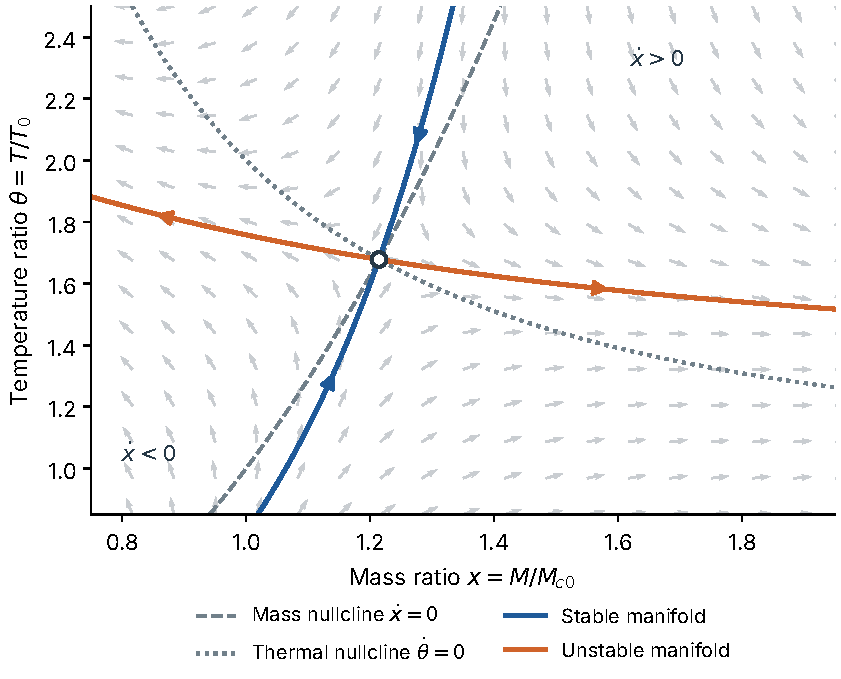
\includegraphics[width=.78\linewidth]{phase_portrait.pdf}
 \caption{\textbf{Phase portrait for $\chi=\zeta=1$.} The mass and thermal nullclines meet at the single equilibrium (open circle). Arrowheads mark the direction of time: the stable manifold (blue) approaches the saddle and the unstable manifold (orange) leaves it. Gray arrows show the direction of the flow.}
 \label{fig:phase}
\end{figure}

\subsection{Parameter scan}
Figure~\ref{fig:scan} shows $\lambda_+$ on a $201\times201$ logarithmic grid with $10^{-2}\le\chi,\zeta\le10^2$. It ranges from 0.20 to 3.98 and depends mainly on $\chi$, which sets the equilibrium mass. On a separate $41\times41$ grid the script also confirms $\det J_*<0$, $\lambda_+>a>0$ and $\lambda_-<-\zeta$ at every point. These scans illustrate Eq.~\eqref{eq:det}; the analytic determinant, not the finite grid, establishes the result for all positive parameters.

\begin{figure}[tbp]
 \centering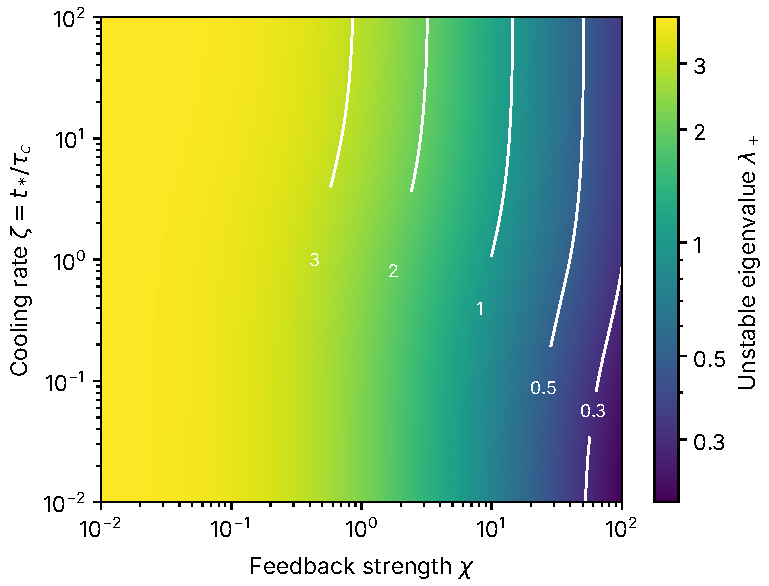
\includegraphics[width=.66\linewidth]{parameter_scan.pdf}
 \caption{\textbf{The unstable eigenvalue over the $(\chi,\zeta)$ plane.} White contours mark constant $\lambda_+$. The eigenvalue decreases with feedback strength but is positive everywhere, as Eq.~\eqref{eq:det} requires.}
 \label{fig:scan}
\end{figure}

\subsection{Equal fractional perturbations}
Figure~\ref{fig:departures} perturbs each model by $\pm2\%$ in mass relative to its own equilibrium: the fixed-medium model from $x=1\pm0.02$ and the coupled model from $(x_*(1\pm0.02),\theta_*)$, both on the time axis $s=t/\tstar$. All four trajectories leave their balance. The coupled ones leave more slowly because the equilibrium mass is larger, in agreement with $\lambda_+<4$.

\begin{figure}[tbp]
 \centering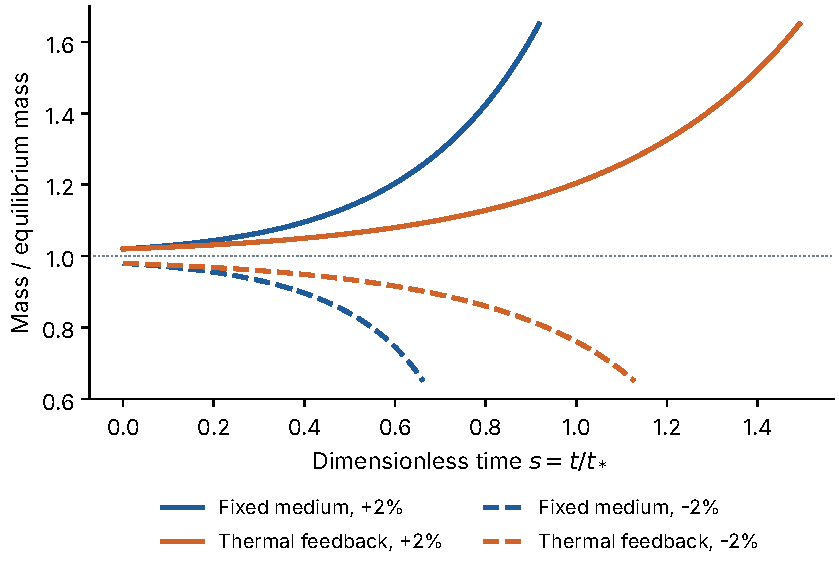
\includegraphics[width=.78\linewidth]{departures.pdf}
 \caption{\textbf{Both balances repel perturbations.} Mass divided by each model's own equilibrium mass after $\pm2\%$ perturbations; the coupled model has $\chi=\zeta=1$ and starts at its equilibrium temperature. Curves end at plotting cutoffs.}
 \label{fig:departures}
\end{figure}

\section{Physical scales}\label{sec:physical}
The saddle result does not depend on material constants, but identifying $T$ with the temperature that sets the Bondi boundary condition does. We test this identification with two fully ionized hydrogen media: a hot plasma with $T_0=10^6$~K and proton density $n=10^{20}\,\mathrm{m^{-3}}$, and a hydrogen medium at the central temperature and density of the Sun, $T_0=1.56\times10^7$~K and $\rho=1.5\times10^5\,\mathrm{kg\,m^{-3}}$~\cite{nasa}. The second case borrows only these two numbers and is not a model of the solar core. In both cases $\gamma=5/3$, $\mu=1/2$ and $\lambda=1/4$.

\subsection{Flow, heating and cooling times}
At the balance mass $\Mc$ we define the Bondi radius $r_B=G\Mc/c_s^2$ and the flow time $t_{\rm flow}=r_B/c_s$. A sphere of radius $r_B$ contains thermal energy $E_B=3nk_BT_0V_B$, with $V_B=4\pi r_B^3/3$. The Thomson optical depth $\tau_T=n\sigma_Tr_B$ estimates the probability that a photon scatters once while crossing it. If every scattered photon gave all of its energy to the gas, the heating rate would be $\tau_T\Pbb(\Mc)$. This upper estimate gives the shortest possible photon heating time,
\begin{equation*}
 t_{{\rm heat},T}=\frac{E_B}{\tau_T\Pbb(\Mc)}.
\end{equation*}
In reality a scattering transfers only part of the photon energy, and the cross section falls below the Thomson value at high energy. Other Hawking particles are not included in this estimate.

For cooling we use optically thin free--free emission of pure hydrogen from the NRL Plasma Formulary~\cite{nrl},
\begin{equation*}
 q_{\rm ff}=1.69\times10^{-38}\,n^2\sqrt{k_BT_0/(1\,{\rm eV})}\ \mathrm{W\,m^{-3}},\qquad
 t_{\rm ff}=\frac{3nk_BT_0}{q_{\rm ff}},
\end{equation*}
with $n$ in $\mathrm{m^{-3}}$. Free--free emission is only one cooling channel, and gas leaving a region of size $r_B$ removes its energy on the time $t_{\rm flow}$ even if it radiates slowly. The ion mean free path $\ell_{ii}=v_{Ti}/\nu_{ii}$ uses the NRL thermal speed $v_{Ti}=(k_BT/m_p)^{1/2}$ and ion collision rate with $\ln\Lambda=10$. Table~\ref{tab:plasma} collects the results.

\begin{table}[tbp]
\centering\small
\caption{Order-of-magnitude scales at the fixed-medium balance mass $\Mc$ for two fully ionized hydrogen media. Only $T_0$ and $n$ are inputs; the other entries follow from the blackbody, Thomson, free--free and NRL collision prescriptions in the text.}
\label{tab:plasma}
\begin{tabular}{@{}lrr@{}}
\toprule
Quantity & Hot plasma & Solar-center hydrogen\\
\midrule
$T_0$ (K) & $1.00\times10^{6}$ & $1.56\times10^{7}$\\
$n$ ($\mathrm{m^{-3}}$) & $1.00\times10^{20}$ & $8.97\times10^{31}$\\
$c_s$ ($\mathrm{m\,s^{-1}}$) & $1.66\times10^{5}$ & $6.55\times10^{5}$\\
$\Mc$ (kg) & $2.96\times10^{14}$ & $8.54\times10^{11}$\\
$r_B$ (m) & $7.19\times10^{-7}$ & $1.33\times10^{-10}$\\
$t_{\rm flow}$ (s) & $4.34\times10^{-12}$ & $2.03\times10^{-16}$\\
$\tau_T$ & $4.78\times10^{-15}$ & $7.92\times10^{-7}$\\
$\tau_T\Pbb(\Mc)$ (W) & $1.94\times10^{-11}$ & $3.87\times10^{2}$\\
$t_{{\rm heat},T}$ (s) & $3.33\times10^{-4}$ & $1.47\times10^{-15}$\\
$t_{\rm ff}$ (s) & $2.64$ & $1.16\times10^{-11}$\\
$\ell_{ii}/r_B$ & $2.1\times10^{6}$ & $3.1$\\
\bottomrule
\end{tabular}
\end{table}

In the hot plasma, $t_{{\rm heat},T}/t_{\rm flow}\simeq7.7\times10^7$; in the denser medium the ratio is still about 7. Free--free cooling is slower than the flow by factors of $6.1\times10^{11}$ and $5.7\times10^4$. Gas therefore crosses the Bondi region long before it is heated or cools radiatively. If the exchange of gas relaxes the reservoir on $\tau_c\sim t_{\rm flow}$, Eq.~\eqref{eq:params} gives photon-only estimates $\chi\approx1.3\times10^{-8}$ and $0.14$, both upper limits. In addition, the ion mean free path exceeds $r_B$ in both media, so even the continuum Bondi flow assumed at the balance mass is not established. The denser case is sensitive to composition, collision physics and the non-blackbody Hawking spectrum, so its numbers are diagnostics, not statements about the Sun.

\subsection{Relation to accretion-powered feedback}
Cantiello et al.~\cite{cantiello} solve time-dependent spherical hydrodynamics with radiative cooling for primordial black holes in stellar cores. They identify a hot-Bondi regime, a bremsstrahlung-cooling regime that drives the flow toward isothermal, and a photon-trapping regime, and find that cooling raises the accretion rate by a factor of about 2--7 relative to adiabatic Bondi. Their black hole has no intrinsic luminosity; the radiation comes from the accreting gas.

This difference reverses the sign of the feedback. In an accretion-powered system, a higher accretion rate produces more radiation and more heating, which then limits accretion: the feedback is negative and tends to regulate the flow. A Hawking-powered system radiates more when its mass decreases, so the same thermal suppression of accretion acts in the direction of the original perturbation. This reversal is the physical origin of the saddle. For the same reason, their quantitative results cannot be used to fix $\epsilon$, $\Cenv$ or $\tau_c$ here.

\subsection{Requirements for a physical interpretation}
Connecting Eq.~\eqref{eq:system} to a real medium would require a collisional mean free path much smaller than $r_B$; heating and thermalization fast enough to change the sound speed at the Bondi radius; a deposition calculation for the actual Hawking spectrum; and an energy budget that includes advection, radiation and density evolution. A comparison of $t_{\rm heat}$, $t_{\rm cool}$ and $t_{\rm flow}$ is necessary but not sufficient. Accordingly, the illustrative choice $\chi=\zeta=1$ in Sec.~\ref{sec:numerics} is not a calibration of either medium in Table~\ref{tab:plasma}.

These requirements suggest a hierarchy of models in which each step adds one physical ingredient (Table~\ref{tab:hierarchy}).

\begin{table}[tbp]
\centering\small
\caption{A hierarchy of Hawking--Bondi models.}
\label{tab:hierarchy}
\begin{tabular}{@{}lll@{}}
\toprule
Model & State variables & Accretion law\\
\midrule
Fixed medium, Ref.~\cite{paperI} & $M$ & $A=\text{const}$\\
Thermal feedback, this paper & $M,\,T$ & $A(T)$\\
Density response & $M,\,T,\,\rho$ & $A(T,\rho)$\\
Radiation hydrodynamics & $M,\,\rho(r),\,T(r),\,v(r)$ & solved from the flow\\
\bottomrule
\end{tabular}
\end{table}

The next step, a density response, adds a third state variable. Proposition~\ref{prop:sign} does not apply to it, so its stability has to be tested anew; a third variable may or may not change the outcome.

\section{Conclusion}
Coupling the Hawking--Bondi mass balance to a heated and cooled reservoir yields a single equilibrium, hotter and more massive than the fixed-medium balance. Its Jacobian determinant, Eq.~\eqref{eq:det}, is negative for all positive feedback and cooling strengths, so the equilibrium is a saddle. The same holds for every one-zone model in which heating decreases with mass, accretion decreases with temperature and cooling increases with temperature. The thermal response is destabilizing: at a given equilibrium it raises the growth rate from $a$ to $\lambda_+$. The lower absolute rate compared with the fixed-medium balance comes from the shift of the equilibrium to larger mass. The physical reason is the sign of the loop: a Hawking-powered hole radiates more as it loses mass, so heating suppresses accretion exactly when accretion is needed.

Timescale estimates for two hydrogen plasmas show that neither supports a one-zone thermal reservoir at its balance mass, because gas crosses the Bondi region faster than it heats or cools. Whether density evolution, spatial transport or realistic emission spectra can change the result remains open; the sign conditions of Proposition~\ref{prop:sign} identify what any such extension must check.

\appendix
\section{Scaling and the strong-feedback limit}\label{app:scaling}
At $\Mc$, $B=A_0\Mc^4$ and $\tstar^{-1}=A_0\Mc$. Substituting $M=\Mc x$, $T=T_0\theta$ and $t=\tstar s$ into Eq.~\eqref{eq:dimensional} gives Eq.~\eqref{eq:system}. The quantity $\epsilon K/(\Cenv T_0\Mc^2)$ has units of inverse time, so $\eta$ and $\chi$ are dimensionless.

For $\chi\gg1$, Eq.~\eqref{eq:equilibrium} gives $\theta_*^{7/4}\sim\chi$ and $x_*\sim\chi^{3/14}$, hence $a=4x_*^{-3}\sim4\chi^{-9/14}$. The off-diagonal product is $bc=3\eta\,\theta_*^{-5/2}x_*^{-1}\sim3\zeta\chi^{-9/14}$. At fixed $\zeta$, $a\to0$ and the positive root of Eq.~\eqref{eq:eigenvalues} behaves as $\lambda_+\sim a+bc/\zeta\sim7\chi^{-9/14}$. This limit is not uniform if $\zeta$ also tends to zero.

\section{Reproducibility}\label{app:repro}
The script \texttt{reproduce.py} requires NumPy, SciPy and Matplotlib. Running \texttt{python reproduce.py} in the paper directory computes the equilibria, Jacobians and eigenvalues, integrates the trajectories, evaluates Tables~\ref{tab:scan} and~\ref{tab:plasma}, regenerates Figs.~\ref{fig:equilibrium}--\ref{fig:departures} and writes \texttt{results.json}. Figure~\ref{fig:loop} is drawn in the \LaTeX\ source; running \texttt{pdflatex main.tex} twice rebuilds the paper. Constants are SI values: $G=6.67430\times10^{-11}\,\mathrm{m^3\,kg^{-1}\,s^{-2}}$, $\hbar=h/2\pi$ with $h=6.62607015\times10^{-34}$~J\,s, $k_B=1.380649\times10^{-23}\,\mathrm{J\,K^{-1}}$, $m_p=1.67262192\times10^{-27}$~kg and $\sigma_T=6.6524587\times10^{-29}\,\mathrm{m^2}$.

\begin{thebibliography}{9}
\bibitem{paperI} E. Anaraly uulu, ``Stability of a Microscopic Black Hole Reactor: Hawking evaporation and a fixed-medium Bondi model,'' manuscript (2026). \url{https://github.com/IPhO-KG/microscopic-black-hole-reactor}.
\bibitem{hawking} S. W. Hawking, ``Particle creation by black holes,'' \emph{Communications in Mathematical Physics} \textbf{43}, 199--220 (1975). \href{https://doi.org/10.1007/BF02345020}{doi:10.1007/BF02345020}.
\bibitem{page} D. N. Page, ``Particle emission rates from a black hole: Massless particles from an uncharged, nonrotating hole,'' \emph{Physical Review D} \textbf{13}, 198--206 (1976). \href{https://doi.org/10.1103/PhysRevD.13.198}{doi:10.1103/PhysRevD.13.198}.
\bibitem{macgibbon} J. H. MacGibbon and B. R. Webber, ``Quark- and gluon-jet emission from primordial black holes: The instantaneous spectra,'' \emph{Physical Review D} \textbf{41}, 3052--3079 (1990). \href{https://doi.org/10.1103/PhysRevD.41.3052}{doi:10.1103/PhysRevD.41.3052}.
\bibitem{bondi} H. Bondi, ``On spherically symmetrical accretion,'' \emph{Monthly Notices of the Royal Astronomical Society} \textbf{112}, 195--204 (1952). \href{https://doi.org/10.1093/mnras/112.2.195}{doi:10.1093/mnras/112.2.195}.
\bibitem{cantiello} M. Cantiello, O. Gottlieb, C. Norton, M. Kleban and K. Van Tilburg, ``Accretion of primordial black holes in stellar interiors,'' arXiv preprint (2026). \href{https://arxiv.org/abs/2606.02726}{arXiv:2606.02726}.
\bibitem{nasa} NASA Marshall Space Flight Center, ``The solar interior,'' \url{https://solarscience.msfc.nasa.gov/interior.shtml} (accessed 30 September 2026).
\bibitem{nrl} A. Beresnyak, \emph{NRL Plasma Formulary}, U.S. Naval Research Laboratory (2023).
\end{thebibliography}

\end{document}
